% Fig. 4  Recorded execution trace for question A17 (single column, drawn at 3.45 in).
% Provenance: evaluation/v3/results/final6_K1_first_and_only.json and
% final6_K3_posthoc_not_heldout.json, entry "A17" (fields: question, sql, sys_value, expected, action,
% confidence, outcome). SQL abbreviated: identifier quotes and the AS alias removed.
\documentclass[border=2pt]{standalone}
% Shared settings for all InsightFlow AI figures (Times, grayscale, sized for IEEE print).
\usepackage[T1]{fontenc}
\usepackage{mathptmx}
\usepackage{tikz}
\usetikzlibrary{positioning,arrows.meta,calc,fit,patterns,shapes.geometric}
\tikzset{
  >={Stealth[length=4pt,width=3.5pt]},
  stage/.style={draw,rounded corners=1.5pt,fill=gray!8,align=center,inner sep=2.5pt,font=\fontsize{7.5}{8.6}\selectfont},
  ext/.style={draw,dashed,rounded corners=1.5pt,align=center,inner sep=2.5pt,font=\fontsize{7.5}{8.6}\selectfont},
  note/.style={align=left,font=\fontsize{7}{8}\selectfont},
  flow/.style={->,thick},
  dflow/.style={->,dashed},
  every node/.append style={execute at begin node={\hyphenpenalty=10000\exhyphenpenalty=10000}},
}

\begin{document}
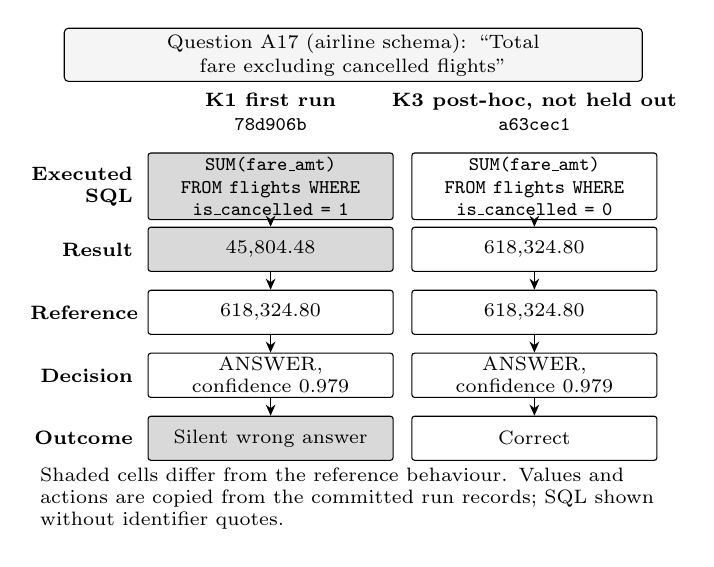
\begin{tikzpicture}[
  lab/.style={align=right,text width=13mm,font=\fontsize{7}{8}\selectfont\bfseries,inner sep=1pt},
  cell/.style={draw,rounded corners=1pt,align=center,text width=30mm,minimum height=5.6mm,inner sep=1.6pt,font=\fontsize{7}{8}\selectfont},
  bad/.style={cell,fill=gray!30}, good/.style={cell,fill=white},
  ]
  \node[draw,rounded corners=1.5pt,fill=gray!8,text width=72mm,align=center,font=\fontsize{7.5}{8.6}\selectfont,inner sep=2pt] (q)
    at (1.05,0.32) {Question A17 (airline schema): ``Total fare excluding cancelled flights''};
  \def\xa{0}\def\xb{3.35}
  \node[font=\fontsize{7.5}{8.6}\selectfont\bfseries,align=center] at (\xa,-0.4) {K1 first run\\\texttt{78d906b}};
  \node[font=\fontsize{7.5}{8.6}\selectfont\bfseries,align=center] at (\xb,-0.4) {K3 post-hoc, not held out\\\texttt{a63cec1}};
  \foreach \r/\l/\a/\b/\sa/\sb in {
    1/{Executed SQL}/{\texttt{SUM(fare\_amt)}\\\texttt{FROM flights WHERE}\\\texttt{is\_cancelled = 1}}/{\texttt{SUM(fare\_amt)}\\\texttt{FROM flights WHERE}\\\texttt{is\_cancelled = 0}}/bad/good,
    2/{Result}/{45{,}804.48}/{618{,}324.80}/bad/good,
    3/{Reference}/{618{,}324.80}/{618{,}324.80}/good/good,
    4/{Decision}/{ANSWER, confidence 0.979}/{ANSWER, confidence 0.979}/good/good,
    5/{Outcome}/{Silent wrong answer}/{Correct}/bad/good} {
    \node[lab] at (-2.4,-0.55-0.8*\r) {\l};
    \node[\sa] (a\r) at (\xa,-0.55-0.8*\r) {\a};
    \node[\sb] (b\r) at (\xb,-0.55-0.8*\r) {\b};
  }
  \foreach \r [evaluate=\r as \n using int(\r+1)] in {1,2,3,4} {\draw[->] (a\r) -- (a\n); \draw[->] (b\r) -- (b\n);}
  \node[note,anchor=north west,text width=80mm] at (-3.05,-4.8) {Shaded cells differ from the reference behaviour. Values and actions are copied from the committed run records; SQL shown without identifier quotes.};
\end{tikzpicture}
\end{document}
